

\documentclass[8pt]{beamer}

% Copyright (C) 2012 - 2013 - EDF R&D - Michael Baudin

\setbeameroption{hide notes}
%\setbeameroption{show notes}
%\setbeameroption{show only notes}
%\mode<presentation>{\usetheme{EDF09}}

\usetheme{EDF09}
\useoutertheme{infolines}

\usepackage[T1]{fontenc}
\usepackage[utf8]{inputenc}
\usepackage{lmodern}

\usepackage[french]{babel}
\uselanguage{French}
\languagepath{French}

% Scilab macros
\newcommand{\sciobj}[1]{\texttt{#1}}
\newcommand{\scifile}[1]{\texttt{#1}}

% Python macros
\newcommand{\pyobj}[1]{\textcolor{blue}{\texttt{#1}}}

\def\RR{\mathbb{R}}
\def\NN{\mathbb{N}}
\def\bx{{\bf x}}

% To highlight source code
\usepackage{listings}
\definecolor{darkgreen}{rgb}{0,0.5,0}
\definecolor{violet}{rgb}{0.5,0,1}
\lstset{
  % general command to set parameter(s)
   basicstyle=\scriptsize\ttfamily, %
   keywordstyle=\color{violet}\bfseries,%
   commentstyle=\color{darkgreen}\bfseries,%
   showspaces=false,%
   stringstyle=\color{red}\bfseries
}

\hypersetup{
    %bookmarks=true,         % show bookmarks bar?
    %unicode=false,          % non-Latin characters in Acrobat�s bookmarks
    %pdftoolbar=true,        % show Acrobat�s toolbar?
    %pdfmenubar=true,        % show Acrobat�s menu?
    %pdffitwindow=false,     % window fit to page when opened
    %pdfstartview={FitH},    % fits the width of the page to the window
    %pdftitle={My title},    % title
    %pdfauthor={Author},     % author
    %pdfsubject={Subject},   % subject of the document
    %pdfcreator={Creator},   % creator of the document
    %pdfproducer={Producer}, % producer of the document
    %pdfkeywords={keyword1} {key2} {key3}, % list of keywords
    %pdfnewwindow=true,      % links in new window
    colorlinks=true,       % false: boxed links; true: colored links
    %linkcolor=red,          % color of internal links (change box color with linkbordercolor)
    %citecolor=green,        % color of links to bibliography
    %filecolor=magenta,      % color of file links
    urlcolor=blue           % color of external links
}

\usepackage{Math_Notations}
\usepackage{color}

\title[Sensitivity analysis]{Sensitivity analysis}

\author[Anne Dutfoy]{
 Anne DUTFOY
}

\institute[]{
 EDF R\&D PERICLES. \\
 anne.dutfoy@edf.Fr
}


\date[PRACE 2021]{PRACE 2021}

%%%%%%%%%%%%%%%%%%%%%%%%%%%%%%%%%%%%%%%%%%%%%%%%%%%%%%%%%%%%%%%%%%%%%%%%%%%%%
\AtBeginSection[]{
  \begin{frame}{Sommaire}
  \small \tableofcontents[currentsection, hideothersubsections]
  \end{frame}
}

  \begin{document}

%%%%%%%%%%%%%%%%%%%%%%%%%%%%%%%%%%%%%%%%%%%%%%%%%%%%%%%%%%%%%%%%%%%%%%%%%%%%%

\begin{frame}[plain]
  \begin{columns}
    \column{0.5\textwidth}
    \column{0.5\textwidth}
    \titlepage
\begin{center}

\includegraphics[height=0.2\textheight]{Maison_Simulation_LOGO.jpg}
\hspace{0.5cm}

\includegraphics[height=0.2\textheight]{PRACE_LOGO.jpg}
\end{center}
    \vfill
  \end{columns}
%\titlepage
\end{frame}

\setbeamertemplate{background canvas}{}

%%%%%%%%%%%%%%%%%%%%%%%%%%%%%%%%%%%%%%%%%%%%%%%%%%%%%%%%%%%%%%%%%%%%%%%%%%%%%




\begin{frame}
  \frametitle{Context}
\small
We consider
\alert{
\begin{align*}
 Y=f(\vect{X})
\end{align*}
}
\begin{itemize}
  \item $f$ is a {\bf model} (scientific simulation software, symbolic function ...)
  \item $\vect{X}=(X_1, \dots, X_d)$ is the set of  {\bf uncertain parameters } modeled by a multivariate distribution of dimension $d$
  \item $Y$ is the {\bf feature of interest} evaluated by the model, supposed here to be scalar.
\end{itemize}

  \begin{block}{Why sensitivity analyses?}
  The main objectives of sensitivity analyses may be:
\begin{enumerate}
 \item \alert{remove some variables} which are not influential on the feature of interest, within a context of high dimension,
 \item\alert{ rank the input variables } in order to focus the modeling on significant inputs: we need a  \emph{relative} quantification
 \item \alert{quantify the impact of a variable}: we need an \emph{exact} quantification
\end{enumerate}
\end{block}
\end{frame}


%%%%%%%%%%%%%%%%%%%%%%%%%%%%%%%%%%%%%%%%%%%%%%%%%
\begin{frame}
\frametitle{Sensitivity: several notions}
\small

Several features can quantify the dependence.

\begin{block}{Sensitivity = Dispersion = Variance}
If we agree that  the \alert{variance is a good way to quantify the dispersion}, sensitivity analyses aim at determining the most important contributors to the variance of $Y$. \\
We use the {\bf conditional expectation}  $\Expect{Y|X_i} = Y^*_i$ which is the random variable function of $X_i$ which approximates $Y$ the best  in the least square sense: 
\begin{align*}
Y^*_i = argmin_{g} \Expect{[Y-g(X_i))]^2}
\end{align*}
No constraint on the nature of the link between $Y$ and $X_i$.\\
\vspace*{0.1cm}

We want to compare  \alert{$\Var{Y^*_i}$} to \alert{$\Var{Y}$}:
 \begin{enumerate}
  \item in the case of independent variables: \alert{Sobol indices},
  \item in the case of dependent variables: importance factors (\alert{Taylor decomposition variance}), \alert{ANCOVA indices}.
 \end{enumerate}
\end{block}

\begin{block}{Sensitivity = \emph{Distance} to the independence}
 If $Y$ and $X_i$ are strongly correlated, the  copula of $(Y,X_i)$ is \emph{far away} from the independent copula.\\
 The \alert{Csiszar divergence measures} enable to quantify that \emph{distance}.
\end{block}

\end{frame}


%%%%%%%%%%%%%%%%%%%%%%%%%%%%%%%%%%%%%%%%%%%%%%%%%

\begin{frame}
  \begin{columns}
    \column{0.4\textwidth}
    \pgfuseimage{sommaire}

    \column{0.6\textwidth}
    {\usebeamercolor[fg]{title page}\huge{Sommaire}}
    \vspace{1cm}
    \small{\tableofcontents}
%\begin{center}
%     \includegraphics[width=0.5\textwidth]{figures/logo-ot}
%\end{center}
  \end{columns}
\end{frame}



%%%%%%%%%%%%%%%%%%%%%%%%%%%%%%%%%%%%%
\section{Independent Variables }



%%%%%%%%%%%%%%%%%%%%%%%%%%%%%%%%%%%%%
\subsection{Sobol Indices}


\begin{frame}
\frametitle{Sobol Indices}
\small

\begin{block}{Variance decomposition}
Generally, if $Y=f(\vect{X})$ and $X$ with {\bf independent components}, then we can decompose the variance as follows: 
\begin{equation}
\label{decompVar}
Var(Y) = \sum_i \Var{\Expect{Y|X_i}} + \sum_{i \neq j} \Var{\Expect{Y|X_i,X_j}} + \dots + \underbrace{\Var{\Expect{Y|X_1,\dots, X_n}}}_{=0}
\end{equation}
\end{block}


\begin{block}{Sobol Indices}
The \alert{\bf Sobol indices of order $k$} quantifies the part of the variance of $Y$ explained by the variance of $(X_{i_1},\dots, X_{i_k})$:

\begin{equation}
\label{SobolOrdrek}
\displaystyle S_{i_1, \dots, i_k} =\frac{\Var{\Expect{Y|X_{i_1}, \dots, X_{i_k}}}}{\Var{Y}}
\end{equation}

The \alert{\bf total Sobol indices of order $k$} quantifies the part of the variance of $Y$ explained by the groups containing the inputs $(X_{i_1},\dots, X_{i_k})$:
\begin{equation}
\label{SobolTotalOrdrek}
\displaystyle S^T_{i_1, \dots, i_k} =\frac{\sum_I\Var{\Expect{Y|X_{I}}}}{\Var{Y}},\, \, \{i_1, \dots, i_k\} \subset I\subset \{1, \dots, n \}
\end{equation}

\end{block}
\end{frame}




%%%%%%%%%%%%%%%%%%%%%%%%%%%%%%%%%%%%%%%%%%%%%%%%%
\begin{frame}
\frametitle{The Hoeffding decomposition}
\small
The  decomposition (\ref{decompVar}) of the  variance of $Y$  comes from the functional Hoeffding decomposition.

\begin{block}{Hoeffding decomposition of a function integrable on $[0,1]^n$}
\textit{If $f$ is integrable on $[0,1]^n$, it admits an unique decomposition which writes: }
\begin{equation}
\label{decompSobol}
\boldsymbol{ f(x_1, \dots, x_n) = f_0 + \sum_{i=1}^{i=n}f_i(x_i) + \sum_{1\leq i < j \leq n} f_{i,j} (x_i, x_j) + \dots + f_{1, \dots, n}(x_1, \dots, x_n)}
\end{equation}
\textit{where} $f_0 = cst$ \textit{and the other functions are mutually orthogonal with respect to the Lebesgue measure on } $[0,1]^n$ :
\begin{equation}
\label{decompSobolCondOrthog}
 \int_0^1 f_{i_1, \dots, i_s}(x_{i_1}, \dots, x_{i_s})f_{j_1, \dots, j_k}(x_{j1}, \dots, x_{j_k}) d\vect{x} = 0
\end{equation}
\textit{as soon as} $(i_1, \dots, i_s) \neq (j_1, \dots, j_k)$.
\end{block}

\end{frame}



%%%%%%%%%%%%%%%%%%%%%%%%%%%%%%%%%%%%%
\begin{frame}
\frametitle{Sobol indices}
\small
How can we use this result for $Y = f(\vect{X})$ with $\vect{X}$ a random vector?

\begin{block}{How can we use this result}
    \small
      We would like to decompose $f$ according to Hoeffding decomposition \dots but: \\
      \begin{enumerate}
      \item  \alert{\bf The inputs of $f$ are not in $[0,1]^n$} :  generally, $Y=f(\vect{X})$ where  $\vect{X}$ is defined on $\mathbb{R}$.
      \end{enumerate}
      \alert{$\Longrightarrow$} If we note
       \begin{equation}
         \label{phi}
         \vect{U} = (F_1(X_1), \dots, F_n(X_n))^t) = \phi^{-1}(\vect{X})
       \end{equation}
       then $\vect{U}$ has uniform marginals and its copula is the same as $\vect{X}$, then {\bf we can use the Hoeffding decomposition on $f \circ \phi$}.

       \begin{enumerate}
       \item  \alert{\bf Are the Sobol indices w.r.t. the  $U_i$ the same as those w.r.t. the $X_i$ ?}
       \end{enumerate}
       \alert{$\Longrightarrow$} If $\vect{U} = \psi(\vect{X})$ where $\psi$ is a diffeomorphism and $Y=f(\vect{X})$ then:

       \begin{equation}
         \label{varCond}
         \Expect{Y|\vect{U}} = \Expect{Y|\vect{X}}
       \end{equation}
       As a matter of fact : $\Expect{Y|\vect{U}} = \Expect{Y|\psi(\vect{X})}$ is the orthogonal projection in a $L_2$ lens of $Y$ on the space generated by $\psi(\vect{X})$, which is the same as the one generated by $\vect{X}$, thus the equality of the random variables  (\ref{varCond}).\\
       As the transformation $\phi$ (\ref{phi}) acts component by component, ($U_i \leftrightarrow X_i$) then we have:
       \begin{equation}
         \label{varCond2}
         \Var{\Expect{Y|U_{i_1}, \dots, U_{i_k}}} = \Var{\Expect{Y|X_{i_1}, \dots, X_{i_k}}}
       \end{equation}
       then {\bf the equality of the Sobol indices w.r.t. the  $U_i$ and to the  $X_i$}.
  \end{block}

\end{frame}




\begin{frame}
  \frametitle{Sobol indices}
\small
  \begin{block}{Probabilistic interpretation of the Hoeffding decomposition}
    \alert{\bf Let's suppose, without loss of generality, that the  $X_i$ are in $[0,1]$}. Then, using the Hoeffding decomposition (\ref{decompSobol}), we have:
    \begin{equation}
      \label{decompSobolY}
      Y = f(\vect{X}) = f_0 + \sum_{i=1}^{i=n}f_i(X_i) + \sum_{1\leq i < j \leq n} f_{i,j} (X_i, X_j) + \dots + f_{1, \dots, n}(X_1, \dots, X_n)
    \end{equation}
    {\bf The orthogonal condition (\ref{decompSobolCondOrthog}) of the  $f_{i_1, \dots, i_k}$  w.r.t. the Lebesgue measure on $[0,1]^n$ can be interpreted as an expectation if the $X_i$ are independent}.\\
    \alert{$\Longrightarrow$} We  suppose now that the $X_i$ are  \alert{\bf independent}.\\

    \alert{\bf Conclusion} :     Y can be decomposed as:
    \begin{equation}
      \label{decompSobolY2}
      \boldsymbol{ Y = f(\vect{X}) = Z_0 + \sum_{i=1}^{i=n}Z_i + \sum_{1\leq i < j \leq n} Z_{i,j}  + \dots + Z_{1,} \dots, n}
    \end{equation}
    where $Z_0 = cst$ et $Z_{i_1, \dots, i_s} \bot  Z_{j_1, \dots, j_k}$ (ie $\Expect{Z_{i_1, \dots, i_s}.Z_{j_1, \dots, j_k}}=0$).
  \end{block}
\end{frame}


\begin{frame}
  \frametitle{Sobol indices}
\small
  \begin{block}{Computation of the Sobol indices}
    \small{
      From the probabilistic decomposition (\ref{decompSobolY2}), we calculate $\Expect{Y}$ and $\Var{Y}$:
      $$
      \left\{
        \begin{array}{l}
          \Expect{Y}  =  Z_0 + \sum_{i=1}^{i=n}\underbrace{\Expect{Z_i}}_{=0 \mbox{ since } \bot Z_0} + \sum_{1\leq i < j \leq n} \underbrace{\Expect{Z_{i,j}}}_{=0 \mbox{ since } \bot Z_0}  + \dots + \underbrace{\Expect{Z_{1,} \dots, n}}_{=0 \mbox{ since } \bot Z_0}  \\[2em]
          \Expect{Y^2}   =   \sum_{I \neq J} \underbrace{\Expect{Z_IZ_J}}_{=0 \mbox{ since } \bot \mbox{ the } Z_I} + \sum_I \Expect{Z_I^2}  \sum_I \Expect{Z_I^2}
        \end{array}
      \right.
      $$
      \begin{eqnarray}
        \label{VarY}
        \Longrightarrow \boldsymbol{\Var{Y} = \sum_{i=1}^{i=n} V_i + \sum_{1\leq i < j \leq n} V_{i,j}  + \dots + V_{1, \dots, n}}
      \end{eqnarray}
      where $V_{i_1, \dots, i_k} = \Var{Z_{i_1, \dots, i_k}} = \Var{f_{i_1, \dots, i_k}(X_{i_1}, \dots, X_{i_k})}$.
    }
  \end{block}
\end{frame}





%%%%%%%%%%%%%%%%%%%%%%%%%%%%%%%%%%%%%
\subsection{An example}


%%%%%%%%%%%%%%%%%%%%%%%%%%%%%%%%%%%%%%%%
\begin{frame}
  \frametitle{An example}
\small
\underline{Data base analysis of aerodynamical coefficients}

\begin{block}{Data}
  \begin{itemize}
  \item We focus on a black box from $\Rset^{24}$ into $\Rset^{12}$
  \item We only know that function through a data base of size $n=377$
  \item We have no information on the distribution followed by the input vector
  \item The objective is to identify, for each output component, the most influential inputs
  \item \alert{We only show the analysis on the first component.}
  \end{itemize}
  \end{block}

\begin{block}{How to proceed?}
  \begin{itemize}
  \item We tested the independence hypothesis of the input using the Spearman coefficients: we can't reject the hypothesis with a level $95\%$
  \item We built a meta model between the output and the inputs, using the penalized chaos polynomial expansion: the model is built from  90\% of the data base and tested on the remaining 10\%
  \item We exploit the model to calculate the Sobol indices (total and of order 1).
  \end{itemize}
\end{block}

\end{frame}


%%%%%%%%%%%%%%%%%%%%%%%%%%%%%%%%%%%%%%%%%%%%%%%%%%%%%%%%%%%%%%%%%%%%%%%%%%%%%%%%%%
\begin{frame}
  \frametitle{Quality of the meta-model}
  \begin{center}
    \resizebox{!}{4cm}{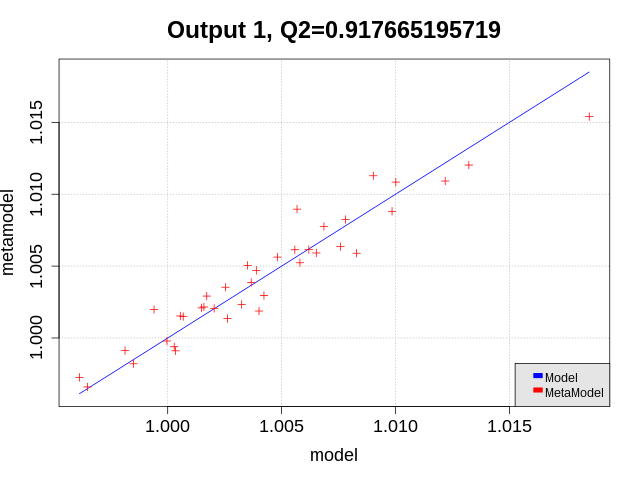
\includegraphics{Figures/Validation_Output_1_q_1.png}}

    Model validation
  \end{center}
\end{frame}

%%%%%%%%%%%%%%%%%%%%%%%%%%%%%%%%%%%%%%%%%%%%%%%%%%%%%%%%%%%%%%%%%%%%%%%%%%%%%%%%%%
\begin{frame}
  \frametitle{Sobol indices}
\small
  \begin{center}
    \resizebox{!}{4cm}{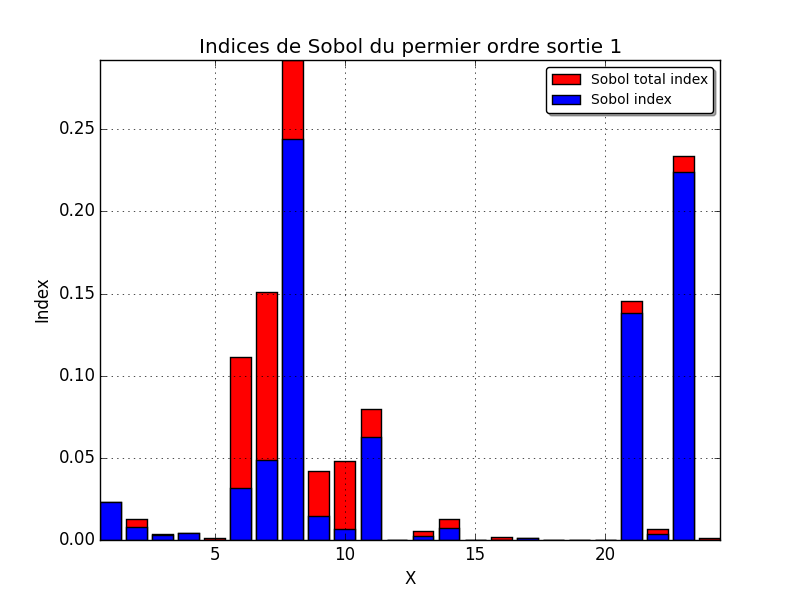
\includegraphics{Figures/Sobol_Output_1.png}}

    Input contributions to the variance of the output
  \end{center}
  We notice that it seems important to keep the inputs 6, 7, 8, 11, 21 et 23, and it is very likely that we can remove the inputs 3, 4, 5, 12, 13, 15, 16, 17, 18, 19, 20, 22 et 24 from the study. Doing that,  we divided  by 2 at least the input dimension.
\end{frame}



%%%%%%%%%%%%%%%%%%%%%%%%%%%%%%%%%%%%%
\subsection{Particular cases: historical measures}

%%%%%%%%%%%%%%%%%%%%%%%%%%%%%%%%%%%%%%%%
\begin{frame}
\frametitle{Historical measures}
 \small
 
 Sobol indices  were introduced by Sobol in 2001 (\cite{Sobol2001}). But sensitivity indices were already existing!:
 \begin{itemize}
  \item SRC, SRRC indices
  \item Pearson, Spearman, PCC, PRCC indices
  \item importance factors from the \emph{Taylor decomposition}
 \end{itemize}
\alert{When the components $X_i$ are independent, these indices are exactly particular cases of Sobol indices.}

 \begin{block}{If the model $f$ is linear  w.r.t. the  $X_i$ : SRC}
  If $\alert{Y = \alpha_0 + \sum_i \alpha_i X_i}$, with \alert{ $X_i$ independent}, then we define the  \alert{ Standard Regression Coefficient (SRC)} :
    \begin{equation}
      SRC(X_i) = \displaystyle \frac{\alpha_i^2 \Var{X_i}}{\Var{Y}}
    \end{equation}
    Then {\bf $SRC $ is the Sobol index} of order 1 of $X_i$ : $\boldsymbol{    SRC (Y / X_i) = S(Y / X_i)}$.
 \end{block}

 
\begin{block}{If the model $f$ is linear  w.r.t. the  $X_i$: Pearson}
 If  \alert{$Y=\alpha_0 + \sum_i \alpha_i X_i$}, then we define the \alert{ Pearson correlation} between $Y$ and $X_i$ as:
   \begin{equation}
    \rho(Y,X_i) =  \dfrac{{\rm cov}\left[Y,X_i \right]}{\sqrt{\Var{X_i}\Var{Y}}} = \dfrac{\Expect{[Y-\Expect{Y}][X_i - \Expect{X_i}]}}{\sqrt{\Var{X_i}\Var{Y}}}
  \end{equation}
Moreover, if the  \alert{ $X_i$ are independent}, we show that:
  $$
  \rho(Y,X_i) = \dfrac{\alpha_i \Var{X_i}}{\sqrt{\Var{X_i}\Var{Y}}} \Longrightarrow (\rho(Y,X_i))^2 = SRC(X_i) = S(Y/X_i)
  $$
  \end{block}
\end{frame}
 
 
 
 

%%%%%%%%%%%%%%%%%%%%%%%%%%%%%%%%%%%%%%%%
\begin{frame}
\frametitle{Historical measures}
 \small
  
 \begin{block}{If the model $rank(f)$ is  linear w.r.t. the $rank(X_i)$: SRRC}
   If $Y = f(\vect{X})$ with \alert{$X_i$ independent}, with $\vect{U} = (F_1(X_1), \dots, F_n(X_n))^t) = \phi^{-1}(\vect{X})$, we have $ Z = F_Y(Y) = F_Y \circ f \circ \phi (\vect{U})$. \\
   

 If we assume  {\bf in addition} that
    \alert{\begin{align}\label{monotone}
           Z = \alpha_0 +\sum_i \alpha_i U_i
           \end{align}
           }
       then we define the  \alert{ Standard Rank Regression Coefficient (SRRC)} :
          $$
     SRRC(Y/X_i) = SRC(Z / U_i) = \dfrac{\alpha_i^2 \Var{U_i}}{\Var{Z}} = S(Z/U_i)
    $$    
       
    Then {\bf SRRC is a Sobol index} of order 1 calculated on the ranks of $X_i$ and $Y$.
           
  \end{block} 

   
 \begin{block}{If the model $rang(f)$ is  linear w.r.t. the ranks $rang(X_i)$: Spearman}
  If we assume that (\ref{monotone}), we define the \alert{ rank Spearman correlation} between $Y$ and $X_i$ as :
  $$
 \rho_S(Y,X_i) = \rho(F_Y(Y),F_i(X_i))
  $$
  As previously, we show that in the case of  \alert{independent variables} :
  $$
  (\rho_S(Y,X_i))^2 = SRRC(Y/X_i) = SRC(Z / U_i) = S(Z/U_i)
  $$
 
\end{block}
 \end{frame}



%%%%%%%%%%%%%%%%%%%%%%%%%%%%%%%%%%%%%%%%
\begin{frame}
\frametitle{Historical measures}

\small
  Importance factors from the \emph{Taylor decomposition} have been defined in metrology first where:
  \begin{itemize}
  \item $Y=f(\vect{X})$
   \item $\vect{X}$ is a gaussian vector with independent components with {\bf low variation coefficient} ($\sigma / \mu \ll 1$)
   \item[$\Longrightarrow$] $f$ is linearised at $\Expect{\vect{X}}$
  \end{itemize}


  \begin{block}{Taylor approximation of order 1 at $\Expect{\vect{X}}$}

$Y=f(\vect{X})$ is approximated by its  \alert{ Taylor approximation of order 1 at $\Expect{\vect{X}}$ } :
\begin{equation}
Y = f[\Expect{\vect{X}}] + <\vect{\nabla }f[\Expect{\vect{X}}], \vect{X} - \Expect{\vect{X}}> =  f[\Expect{\vect{X}}] + \sum_i [X_i-\Expect{\vect{X}_i}]\left.\frac{\partial f}{\partial X_j}\right|_{\Expect{\vect{X}}}
\end{equation}
Under the  {\bf assumption of a linear model at} $\Expect{\vect{X}}$, and  \alert{independent $X_i$}, we have :
\begin{eqnarray}
\Var{Y} & = & \sum_i \left(\left.\frac{\partial f}{\partial X_j}\right|_{\Expect{\vect{X}}}\right)^2 \Var{X_i}
\end{eqnarray}
We define the  \alert{importance factor of $X_i$} :
$$
\boldsymbol{
FI(X_i) = \left(\left.\frac{\partial f}{\partial X_j}\right|_{\Expect{\vect{X}}}\right)^2 \frac{\Var{X_i}}{\Var{Y}}
} = SRC(Y / X_i) = S(Y/X_i)
$$
{\bf The $FI$ are Sobol indices of order 1}.
  
\end{block}

  \end{frame}





%%%%%%%%%%%%%%%%%%%%%%%%%%%%%%%%%%%%%
\section{Dependent variables}

%%%%%%%%%%%%%%%%%%%%%%%%%%%%%%%%%%%%%
\subsection{Taylor decomposition}

%\begin{frame}
%\tableofcontents[currentsubsection]
%\end{frame}


%%%%%%%%%%%%%%%%%%%%%%%%%%%%%%%%%%%%%%%%
\begin{frame}
\frametitle{Taylor decomposition}
\small
In the case of dependent $X_i$, {\bf we  take into account the covariance matrix only} in order to calculate :
\begin{itemize}
 \item the importance factors from the Taylor decomposition
 \item the ANCOVA indices
\end{itemize}

  \begin{block}{Taylor decomposition}
 $Y=f(\vect{X})$ is approximated by its  \alert{ Taylor approximation of order 1 at  $\Expect{\vect{X}}$} :
\begin{equation}
Y = f[\Expect{\vect{X}}] + <\vect{\nabla }f[\Expect{\vect{X}}], \vect{X} -\Expect{\vect{X}}> =  f[\Expect{\vect{X}}] + \sum_i [X_i-\Expect{X_i}]\left.\frac{\partial f}{\partial X_j}\right|_{\Expect{\vect{X}}}
\end{equation}
Under the  {\bf assumption of a linear model at} $\Expect{\vect{X}}$, we have :
\begin{eqnarray}
\Var{Y} & = & \strut^t \vect{\nabla }f[\Expect{\vect{X}}].\mat{\rm Cov}\left[ \vect{X} \right]. \vect{\nabla }f[\Expect{\vect{X}}] = \sum_{i,j} \displaystyle \left.\frac{\partial f}{\partial X_i}\right|_{\Expect{\vect{X}}}{\rm Cov} \left[ X_i, X_j \right].\left.\frac{\partial f}{\partial X_i}\right|_{\Expect{\vect{X}}}
\end{eqnarray}
We define the  \alert{ importance factor of $X_i$} as :
\begin{equation}
\label{FI}
\boldsymbol{FI(X_i) = \displaystyle \frac{\left(\sum_{j} \left.\frac{\partial f}{\partial X_j}\right|_{\Expect{\vect{X}}}{\rm Cov} \left[ X_i, X_j \right]\right)  \left.\frac{\partial f}{\partial X_i}\right|_{\Expect{\vect{X}}}}{\Var{Y}}}
\end{equation}
\end{block}

\end{frame}



%%%%%%%%%%%%%%%%%%%%%%%%%%%%%%%%%%%%%
\subsection{ ANCOVA Indices}

\begin{frame}
  \frametitle{ANCOVA indices}
\small

The  \alert{ANCOVA} (ANalysis of COVAriance) method, is a variance-based method generalizing the ANOVA (ANalysis Of VAriance) decomposition for models with correlated input parameters (see \cite{Caniou2012}).\\
It is based on the Hoeffding decomposition of $f$ that writes:
\begin{equation}
 Y = f(x_1, \dots, x_n) = f_0 + \sum_{U \subset \{ 1, n\}} f_U(\vect{X}_U)
\end{equation}
where $U$ is a non empty set of indices in $\{ 1, n\}$. Thus $f_U(\vect{X}_U)$ is the combined contribution of  $X_U$ to $Y$.

\begin{block}{Definition}
The total part of variance of $Y$ due to $\vect{X}_U$ writes:
\begin{align*}
 \alert{S_U = \dfrac{\Cov{Y, f_U(\vect{X}_U)}}{\Var{Y}} = S_U^{1} + S_U^{2}}
\end{align*}
 where
$$
 \left\{
 \begin{array}{lcl}
  S_U^{1} & = & \dfrac{\Var{f_U(\vect{X}_U)}}{\Var{Y}} \\[1em]
  S_U^{2} & = & \dfrac{\Cov{f_U(\vect{X}_U), \sum_{V | V \cap U = \emptyset} f_V(\vect{X}_V)}}{\Var{Y}}
  \end{array}
  \right.
$$

\alert{
$S_U^{1}$ is the contribution to $\Var{Y}$ of $\vect{X}_U$.\\
$S_U^{1}$ is the contribution to $\Var{Y}$ of $\vect{X}_U$ through its correlation to the other variables.
}
\end{block}

\end{frame}




%%%%%%%%%%%%%%%%%%%%%%%%%%%%%%%%%%%%%
\section{Extensions}

\subsection{Indices based on the Csiszar divergence}

\begin{frame}
 \frametitle{Csiszar Divergence}
\small
\underline{Principle}: The sensitivity of $Y$ w.r.t. $X_i$ is no more defined as the part of the variance of $Y$ due to the variance of $X_i$. We use a notion of distance between the real dependence between $Y$ and $X_i$, and the independence.\\
We assume that $Y$ and $X_i$ are scalar to ease the notations of this presentation.

\begin{block}{Indices based on the Csiszar divergence}
 In \cite{Borgonovo2016} and \cite{DaVeiga2013} , the authors compare the distribution of  $(X_i,Y)$, with pdf $p_{X_i,Y}$ to the product distribution of $X_i$ and $Y$ (which assumes the independence), with pdf $p_{Y}\otimes p_{X_i}$. \\
 They define some sensitivity indices based on the  \alert{Csiszar divergence $D_f$} as:
    \begin{align*}
      S_i^f= D_f(p_{Y \otimes X_i} \| p_{(Y,X_i)})
    \end{align*}
 We show that this index: 
 \begin{itemize}
  \item depends on the whole distribution and not on its first moments only
  \item is independent of the margins (and then of the scale of the components)
 \end{itemize}
This indice  depends on the copula only as it can be written as:
    \alert{\begin{align*}
      S_i^f= D_f(\Pi \| c_{(Y,X_i)})
    \end{align*}}

\end{block}

\underline{Recall}: The copula of $(X,Y)$ is the same as the copula of $(f(X), g(Y))$ if $f$ and $g$ are some increasing functions.\\
In particular, we can consider the uniform margins with  $f = F_X$ and $g = F_Y$.
\end{frame}



%%%%%%%%%%%%%%%%%%%%%%%%%%%%%%%%%%%%%



\begin{frame}
  \frametitle{CsiszarDivergence}
\small
  \begin{block}{D\'efinition}
(\cite{Csiszar1963})
    Let $P$ and $Q$ be two probability measures defined on the space $\Omega$ and  $f$ a  convex positive function defined at least on $\Rset^+$ such that $f(1)=0$.\\
    The $f$-Csisz\'ar divergence of $Q$ w.r.t. $P$ is defined as:
    \begin{itemize}
     \item If $P$ and $Q$ are absolutely continuous w.r.t. the Lebesgue measure $dx$, with pdf $p$ and $q$, and if $P  \ll Q$, then: 
    \begin{align}
     \alert{ D_f(P||Q)=\int_{\Omega}f\left(\dfrac{p(x)}{q(x)}\right)q(x)dx} \quad \in[0,+\infty]
    \end{align}
    \item If $P$ and $Q$ are absolutely continuous w.r.t. the counting measure defined on the $(x_k)_{k \in \Nset}$ (Dirac) and if $P  \ll Q$, then:
    \begin{align}
     \displaystyle D_f(P||Q)=\sum_{k=0}^{\infty}f\left(\dfrac{p(x_k)}{q(x_k)}\right)q(x_k)     
    \end{align}

    \end{itemize}
    
    
    \end{block}
    \underline{Recall}: $P  \ll Q$ means $q(x)= 0 \Longrightarrow p(x)=0$
\end{frame}



%%%%%%%%%%%%%%%%%%%%%%%%%%%%%%%%%%%%%
\begin{frame}
  \frametitle{Examples}
\centering
      \begin{tabular}{lccc}
        \hline\noalign{\smallskip}
        Name & Formula & Generator $f(u)$ & $f(0)+f^*(0)$ \\
        \noalign{\smallskip}\hline\noalign{\smallskip}
        Total Variation & $\displaystyle\dfrac{1}{2}\int|p(x)-q(x)|dx$ & $\displaystyle\dfrac{1}{2}|u-1|$ & 1 \\
        Kullback-Liebler & $\displaystyle\int p(x)\log\dfrac{p(x)}{q(x)}dx$ & $\displaystyle-\log u$ & $\infty$ \\
        Hellinger (square) & $\displaystyle\int\left(\sqrt{p(x)}-\sqrt{q(x)}\right)^2dx$ & $\displaystyle\left(\sqrt{u}-1\right)^2$ & 2 \\
        Chi-2 Pearson & $\displaystyle\int\dfrac{\left(p(x)-q(x)\right)^2}{p(x)}dx$ & $\displaystyle(u-1)^2$ & $\infty$ \\
        \noalign{\smallskip}\hline \\[0.5em]
      \end{tabular}
 \\
 where $f^*:u\mapsto uf(1/u)$ the function $*$-conjugate of $f$
\end{frame}



%%%%%%%%%%%%%%%%%%%%%%%%%%%%%%%%%%%%%
\begin{frame}
  \frametitle{Examples}
\begin{block}{Properties}
  \begin{itemize}
  \item Unicity: $\forall (P,Q), D_{f_1}(P||Q)=D_{f_2}(P||Q) \Leftrightarrow \exists c\in\Rset, f_1(u)-f_2(u)=c(u-1)$ 
  \begin{itemize}
  \item The divergences $D_{f_1}$ and $D_{f_2}$  quantify the gaps between the distributions  exactly the same way when  $f_1$ and $f_2$ differ from a linear function of $(u-1)$
  \item The divergences based on Kullback-Liebler and Hellinger are different
  \end{itemize}
  \item Symmetry: $\forall (P,Q), D_{f}(P||Q)=D_{f^*}(Q||P)$ and $\forall (P,Q),D_{f^*}(P||Q)=D_{f}(P||Q)\Leftrightarrow \exists c\in\Rset, f^*(u)-f(u)=c(u-1)$
  \item Range: \alert{$\displaystyle 0=f(1)\leq D_f(P||Q)\leq f(0)+f^*(0)$}
  \item Convexity: $\displaystyle \forall \lambda\in[0,1],\quad D_f(\lambda P_1+(1-\lambda)P_2||\lambda Q_1+(1-\lambda)Q_2)\leq\lambda D_f(P_1||Q_1)+(1-\lambda)D_f(P_2||Q_2)$
  \end{itemize}
  \end{block}

  \end{frame}


%%%%%%%%%%%%%%%%%%%%%%%%%%%%%%%%%%%%%%%%%%%%%%%%%%%%%%%%%%%%%%%%%%%%
\begin{frame}
  \frametitle{Csiszar Divergence}
\small
The sensitivity index writes:
    \begin{align*}
      S_i^f= D_f(\Pi \| c_{(Y,X_i)}) = \int_{[0,1]^2}f\left(\dfrac{1}{c_{X_i,Y}(u,v)}\right)c_{X_i,Y}(u,v)\,dudv=\int_{[0,1]^2}f^*\left(c_{X_i,Y}(u,v)\right)\,dudv
    \end{align*}

  \begin{block}{How to interpret these indices?}
  \begin{itemize}
   \item \alert{If $Y \perp X_i$ then $S_i^f=0$}  (equivalence if $f$ is strictly convex). In that case, $X_i$ can be removed from the study since it has no impact on  $Y$.
   \item \alert{If $Y=f(X_i)$ then $S_i^f = f(0) + f^*(0)$}.
  \end{itemize}
The characterisation of the range of the indices is the main result for the dependence analysis.
  \end{block}

  \begin{block}{Methodology and numeric issues}
   Works are in progress on the following challenges: 
    \begin{itemize}
    \item \alert{how to interpret the value of the sensitivity index?} $S_i^f=0.8$: if if is a Sobol' index, it means that $80\%$ of the variance of $Y$ is explained by the variance of $X_i$... but what if Csiszar divergence?
    \item \alert{which  $f$ to consider?} If $S_i^{f} > S_j^{f}$, do we still have $S_i^{g} > S_j^{g}$? Answer: no... thus, the ranking depends on $f$. We have to \emph{adapt $f$} to the needs of the study. For example, if $c(x_i, y)$ is low in some particular zones, we take a $f$ which increases the gaps to 1 in that zone. We need to build a know-how!
      \item \alert{how to estimate a copula density $c_{(Y,X_i)}$}:  $\hat{S}_i^f = S_i^f(\hat{c})$ $\Longrightarrow$ use of the Bernstein copula?
     \item \alert{how to create independence tests} based on an estimation of $S_i^f$, according to $f$?: under the independence assumption, which confidence interval do we have on the values of $\hat{S}_i^f$?
    \end{itemize}

  \end{block}

\end{frame}

%%%%%%%%%%%%%%%%%%%%%%%%%%%%%%%%%%%%%%%%%%%%%%%%%%%%%%%%%%%%%%%%%%%%
\begin{frame}
  \frametitle{Csiszar Divergence - Independence Test}
  \small
  
  \begin{block}{Proposition I}
   How to proceed: 
   \begin{enumerate}
    \item On the sample $k$ of $(x_i, y)$ of size $n$, generated under the independence assumption between $x_i$ and $y$, we build the copula density $\hat{c}_k(x_i,y)$  of $(x_i,y)$ thanks to the Bernstein copula;
    \item We repeat Step 1  $N$ times: we draw, at any point $(x_i,y)$, the quantiles $5\%$ and $95\%$ of the values of $\hat{c}_k(x_i,y), 1\leq k \leq N$;
    \item We build \alert{$90\%$ confidence domain} point by point.
   \end{enumerate}
From the new sample to be tested, we build the copula density: if it goes out of the confidence domaine, then we reject the independence assumption.
  \end{block}

 \underline{Example}: Copula of $(X_{19}, Y_1)$ (left) and of $(X_8, Y_1)$ (right)
\begin{center}
    \resizebox{5cm}{!}{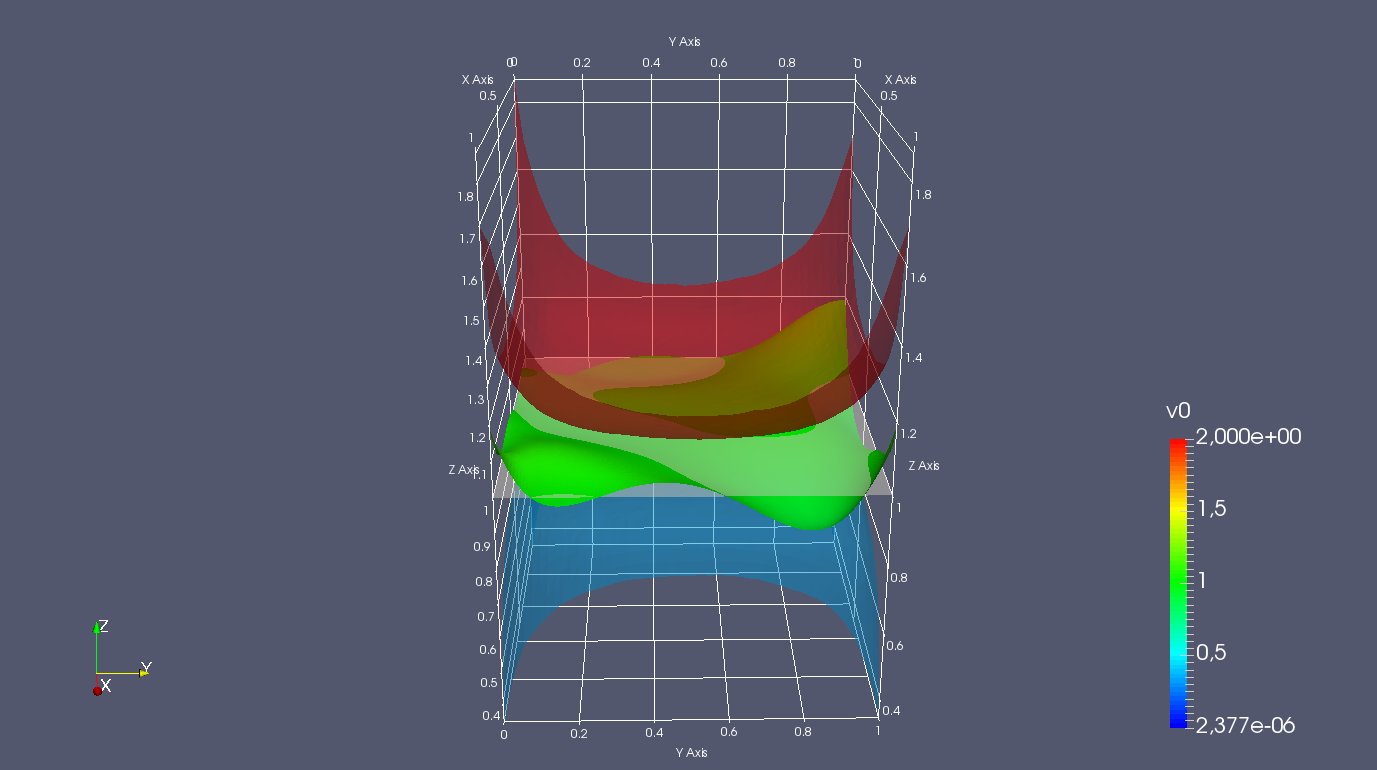
\includegraphics{Figures/Output_1_input_19.png}}\, \resizebox{5cm}{!}{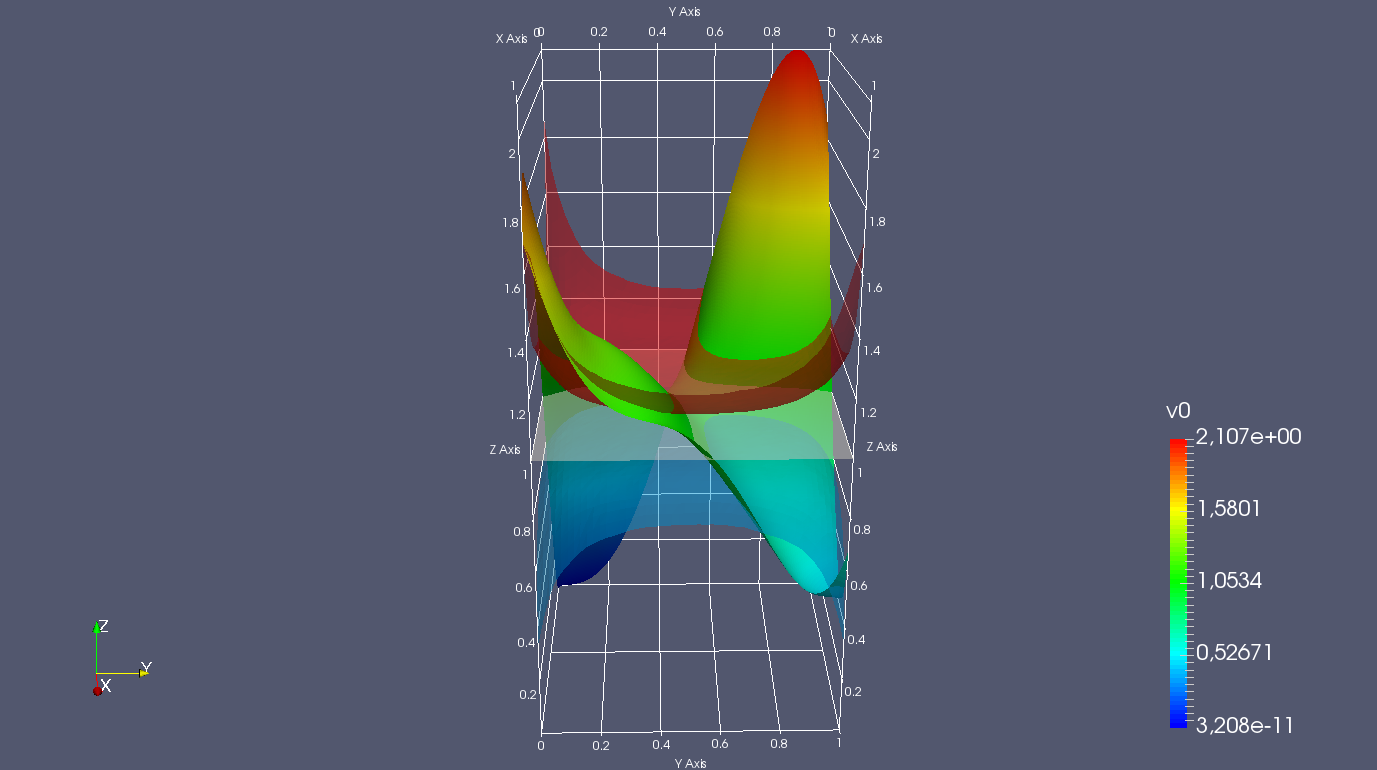
\includegraphics{Figures/Output_1_input_8b.png}}
  \end{center}
  These graphs show that we can't reject the assumption that $Y_1$ is independent from $X_{19}$, while $Y$ is clearly highly dependent on $X_8$.
  \end{frame}
  
  
  
%%%%%%%%%%%%%%%%%%%%%%%%%%%%%%%%%%%%%%%%%%%%%%%%%%%%%%%%%%%%%%%%%%%%
\begin{frame}
  \frametitle{Csiszar Divergence - Independence Test}
  \small
  
  \begin{block}{Proposition II}
   According to the previous procedure, we calculate $\hat{S}_i ^f = S_i^j(\hat{c})$ for each $f$ and  we determine a distribution of $\hat{S}_i ^f$ and a confidence interval under the independence assumption.
  \end{block}

 \underline{Example}: Estimation of sensitivity indices, $n=1000$, $N = 10^4$.
 \begin{center}
    \resizebox{4.1cm}{!}{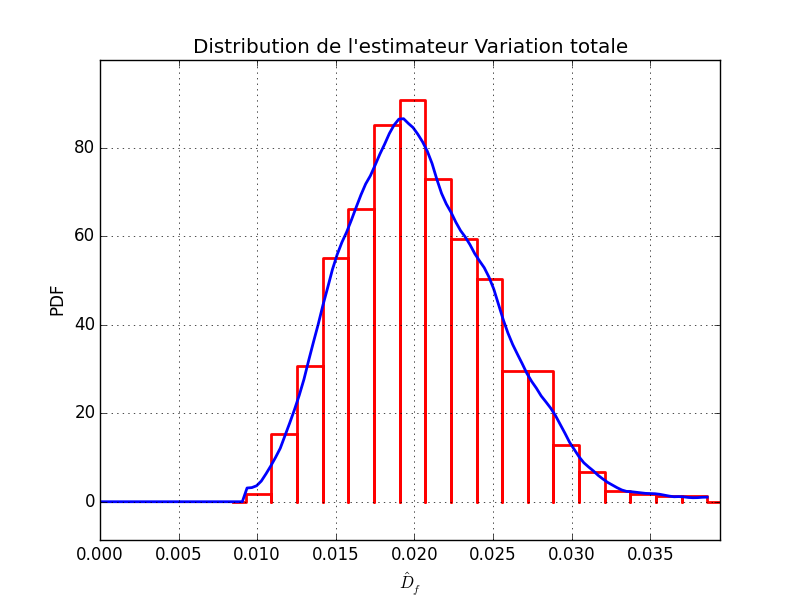
\includegraphics{Figures/sensitivity_0.png}}\,
    \resizebox{4.1cm}{!}{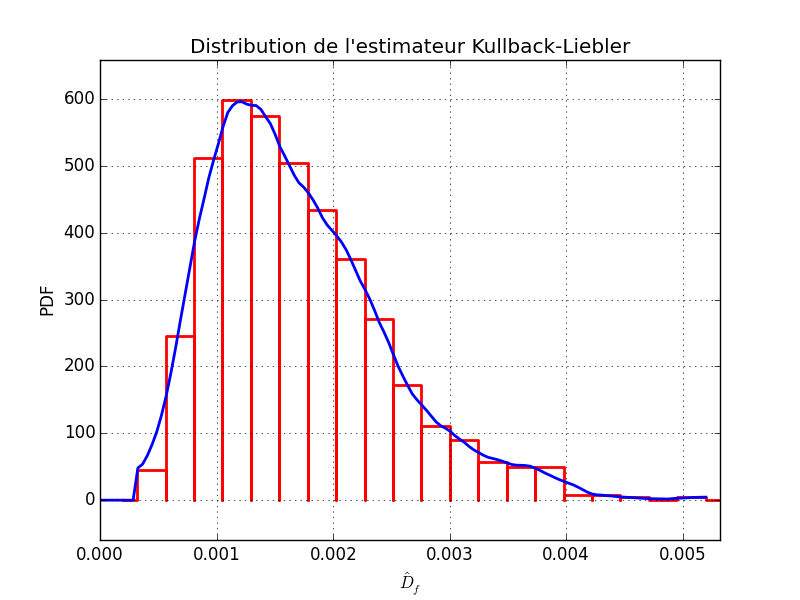
\includegraphics{Figures/sensitivity_1.png}}\\[0.1em]
    \resizebox{4.1cm}{!}{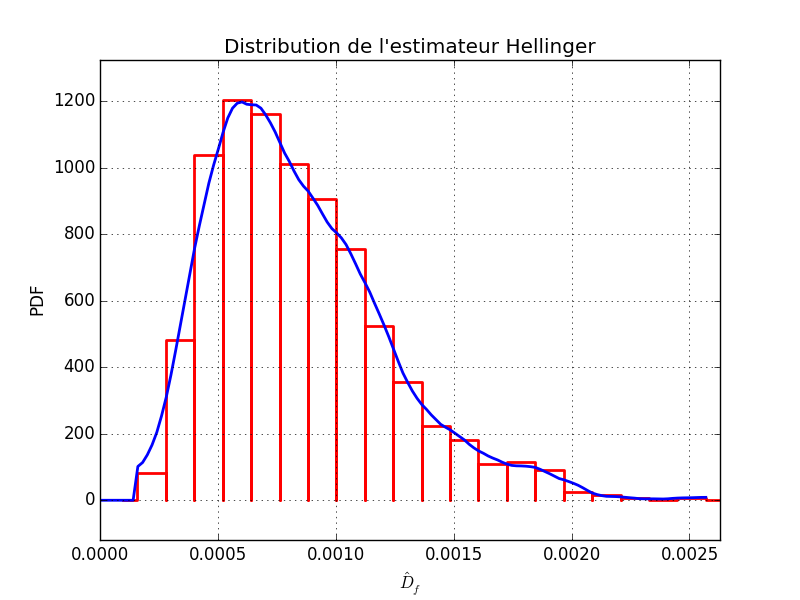
\includegraphics{Figures/sensitivity_2.png}}\,
    \resizebox{4.1cm}{!}{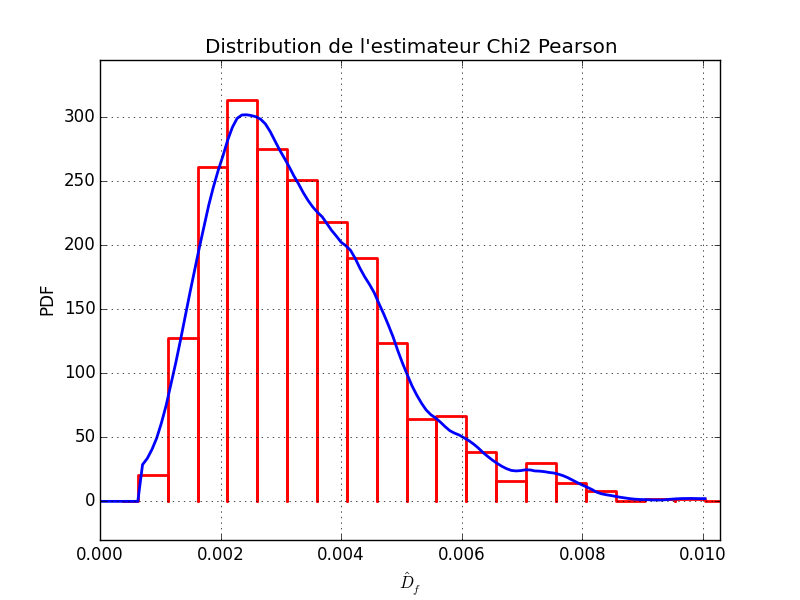
\includegraphics{Figures/sensitivity_3.png}}\\[0.1em]
    
  \end{center}
  \end{frame}
  
  
%%%%%%%%%%%%%%%%%%%%%%%%%%%%%%%%%%%%%
\section{References}

\begin{frame}[allowframebreaks]
  \frametitle{R\'ef\'erences}
  \bibliographystyle{abstract} % style alphabétique en anglais
  \bibliography{bibliothese} % pour afficher la biblio
\end{frame}



\end{document}
